\documentclass{beamer}

\usepackage{amssymb,amsmath}
\usepackage{graphicx}
\usepackage{url}
\usepackage{color}
\usepackage{pagenote}[continuous,page]
\usepackage{relsize}		% For \smaller
\usepackage{url}			% For \url
\usepackage{epstopdf}	% Included EPS files automatically converted to PDF to include with pdflatex

%For MindMaps
% \usepackage{tikz}%
% \usetikzlibrary{mindmap,trees,arrows}%

%%% Color Definitions %%%%%%%%%%%%%%%%%%%%%%%%%%%%%%%%%%%%%%%%%%%%%%%%%%%%%%%%%
%\definecolor{bordercol}{RGB}{40,40,40}
%\definecolor{headercol1}{RGB}{186,215,230}
%\definecolor{headercol2}{RGB}{80,80,80}
%\definecolor{headerfontcol}{RGB}{0,0,0}
%\definecolor{boxcolor}{RGB}{186,215,230}

%%% Save space in lists. Use this after the opening of the list %%%%%%%%%%%%%%%%
%\newcommand{\compresslist}{
%	\setlength{\itemsep}{1pt}
%	\setlength{\parskip}{0pt}
%	\setlength{\parsep}{0pt}
%}

%\setbeameroption{show notes on top}

% You should run 'pdflatex' TWICE, because of TOC issues.

% Rename this file.  A common temptation for first-time slide makers
% is to name it something like ``my_talk.tex'' or
% ``john_doe_talk.tex'' or even ``discrete_math_seminar_talk.tex''.
% You really won't like any of these titles the second time you give a
% talk.  Try naming your tex file something more descriptive, like
% ``riemann_hypothesis_short_proof_talk.tex''.  Even better (in case
% you recycle 99% of a talk, but still want to change a little, and
% retain copies of each), how about
% ``riemann_hypothesis_short_proof_MIT-Colloquium.2000-01-01.tex''?

\mode<presentation>
{
  \usetheme{CambridgeUS}		% bem bacana - menu superior
  \usecolortheme{default}		% branco, azul clarinho
  \useoutertheme{default}
  \useinnertheme{circles}
  \setbeamercovered{invisible}
}

\beamertemplatenavigationsymbolsempty

%% Better looking blocks
\setbeamercolor{block title alerted}{use=structure,fg=black,bg=red!80!black}
\setbeamercolor{block body alerted}{use=structure,fg=black,bg=white!90!black}

\setbeamercolor{block title}{use=structure,fg=black,bg=blue!60!white}
\setbeamercolor{block body}{use=structure,fg=black,bg=white!90!black}

\usepackage[english]{babel}
\usepackage[latin1]{inputenc}
\usepackage{subfigure}

\usepackage{times}
\usepackage[T1]{fontenc}

%% makes the ppagenote command for figure references at the end.
\makepagenote
\renewcommand{\notenumintext}[1]{}
\newcommand{\ppagenote}[1]{\pagenote[Page \insertframenumber]{#1}}


\usepackage{tikz}
\usetikzlibrary{arrows,shapes}

\title[GB13604]{GB13604 - Maths for Computer Science}
\subtitle[]{Lecture 8 -- Probability, Part I}
\author[Claus Aranha]{Claus Aranha\\{\footnotesize caranha@cs.tsukuba.ac.jp}}
\institute[COINS]{College of Information Science}
\date[2018-11-21]{2018-11-21\\{\tiny Last updated \today}}

\tikzstyle{vertex}=[circle,fill=black!25,minimum size=10pt,inner sep=0pt]
\tikzstyle{blue vertex}=[circle,fill=blue!100,minimum size=10pt,inner sep=0pt]
\tikzstyle{red vertex}=[circle,fill=red!100,minimum size=10pt,inner sep=0pt]
\tikzstyle{yellow vertex}=[circle,fill=yellow!100,minimum size=10pt,inner sep=0pt]
\tikzstyle{edge} = [draw,thick,-]
\tikzstyle{pedge} = [draw,thick,.]
\tikzstyle{red edge} = [draw, thick,-,red!50]
\tikzstyle{black edge} = [draw, line width=2pt,-,black!20]
\tikzstyle{weight} = [font=\smaller]

\begin{document}

\begin{frame}
  \maketitle

  \begin{center}
    {\smaller This course is based on Mathematics for Computer Science, Spring
    2015, by Albert Meyer and Adam Chlipala, Massachusetts Institute
    of Technology OpenCourseWare.}
    
    
\includegraphics[width=0.2\textwidth]{../img/by-nc-sa}
  \end{center}
\end{frame}

\section{Introduction}

\begin{frame}
  \frametitle{Last Topic: Probability}

  {\larger

    Probability is absolutely essential to the Engineering, Sciences,
    and Social studies. And it is also very important to understand in
    daily life as well.

    \bigskip

    \begin{itemize}
    \item Probability as the study of gambling (Lottos, Casinos,
      Gatchas).
      \bigskip
      
    \item Probability for Extrapolating information about society
      (Chances of Death and Sickness, Insurance, Average behavior of
      populations)
      \bigskip
      
    \item Probability for the analysis of Noisy Data and Noisy Processes.
      (Stochastic Algorithms, Experiments, Resilience Engineering)
    \end{itemize}
  }
\end{frame}

\begin{frame}
  \frametitle{Unit Goals and Outline}
  {\larger

    \begin{itemize}
    \item Discrete Probability
    \item Conditional Probability
    \item \alert{Independence and Causality}
    \item \alert{Random Variables and Density Functions}
    \item \alert{Expectation}
    \item \structure{Deviation}
    \item \structure{Sampling and Confidence}
    \item \structure{Random Walks}
    \end{itemize}

  }
\end{frame}

\section{Discrete Probability}

\subsection{Probability as counting}
\begin{frame}
  \frametitle{Poker Example: Probability of Two Jacks}

  \hfill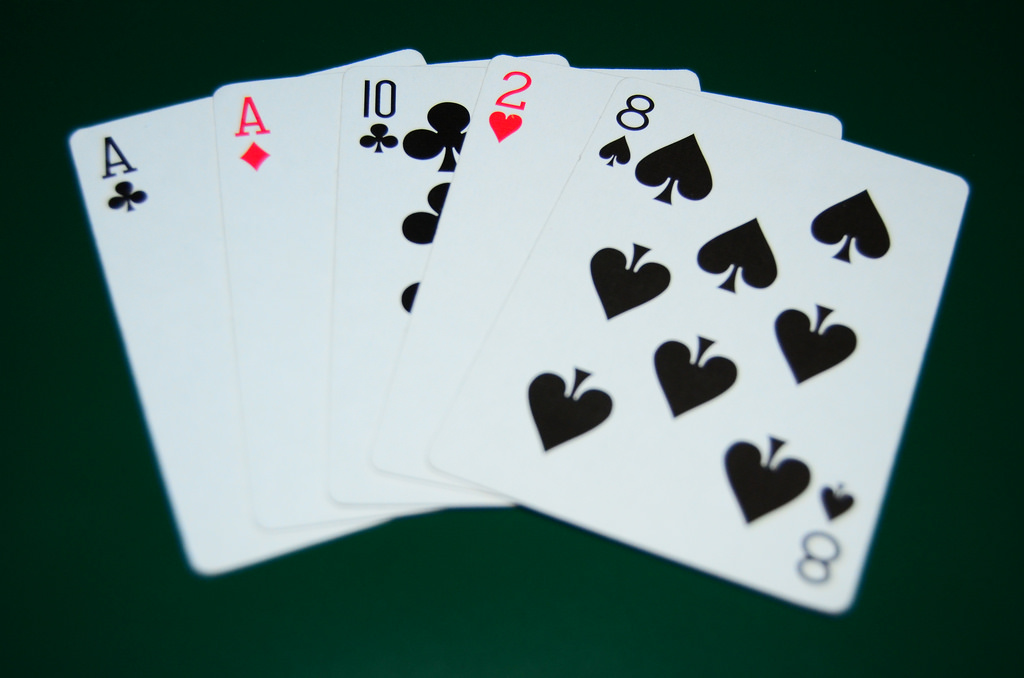
\includegraphics[width=0.2\textwidth]{../img/poker_pair}
  
  {\larger

    What is the probability of getting \structure{exactly two aces}
    in a poker hand?

    \bigskip

    This can be seen as a counting problem:
    \begin{itemize}
    \item <2->All outcomes: $\binom{52}{5}$ sets of 5 cards
    \item <3->Desired outcomes: $\binom{4}{2}\binom{52-4}{5-2}$ two ace hands.
    \item <4->Probability: Desired outcome/All outcomes = $\frac{\binom{4}{2}\binom{48}{3}}{\binom{52}{5}}$
    \item <4-> (About 0.04)
    \end{itemize}
  }
\end{frame}

\begin{frame}
  \frametitle{Probability as a counting problem}

  {\larger
    {\bf Basic Idea}: ``What fraction of the time do I get what I want?''

    \bigskip
    
    \begin{equation*}
      \text{Pr(event)} = \frac{\text{Outcomes we want}}{\text{All possible outcomes}}
    \end{equation*}
  }
\end{frame}

\begin{frame}
  \frametitle{Probability as a counting problem: nomenclature}

  {\larger
    \begin{itemize}
    \item A set of experimental {\bf \structure{outcomes}}
      \bigskip
      
    \item A subset of outcomes is an {\bf \structure{event}}
      \bigskip

    \item Probability of an event:\\
      \begin{equation*}
        \text{Pr(event)} = \frac{\text{\# outcomes in the
            event}}{\text{total \# of outcomes}}
      \end{equation*}
      
    \end{itemize}

    \vfill

    Applies to a lot of cases (but not all of them)
  }  
\end{frame}

\subsection{Monty Hall Problem}

\begin{frame}
  \frametitle{The Monty Hall Problem}
  {\larger

    \begin{itemize}
    \item 1970's American TV sholl \structure{``Let's make a Deal''}\\
      \hfill(Hosted by Monty Hall)

      \begin{center}
        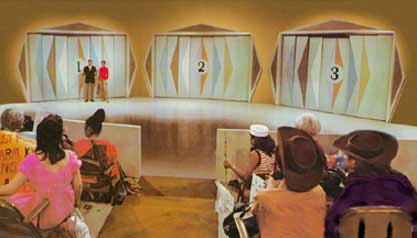
\includegraphics[width=0.6\textwidth]{../img/montyhall}
      \end{center}
      
    \item One door has a good prize (a car?) and two doors have a bad
      prize (a goat?)
    \end{itemize}
  }  
\end{frame}

\begin{frame}
  \frametitle{Rules of the Monty Hall Problem}

  {\large
    \begin{itemize}
    \item Goats behind two doors, car behind one door;
    \item Contestant \alert{chooses a door};
    \item Monty \structure{reveals a door} with a goat behind it;
    \item Contestant choose to \alert{stick or switch} doors;
    \end{itemize}
    \vfill
    
    Mary Savant published a column in a science magazine about the
    game that sparked a debate on two positions:
    \begin{enumerate}
    \item \alert{stick and switch} are equally good
    \item \alert{switch} is much better than \alert{stick}
    \end{enumerate}
  }
\end{frame}

\begin{frame}
  \frametitle{Analysing Monty Hall}

  {\large
    \begin{itemize}
    \item What are the outcomes? What is the event?
      \bigskip
      
    \item We will use a \alert{probability tree} to analyse the game
      step by step and define these sets.
    \end{itemize}
  }
\end{frame}

\begin{frame}
  \frametitle{Analysis: Switch Strategy}

  {\large
    \alert{Switch: Pick a door, Reveal Goat, Switch Door}

    \begin{columns}
      \column{0.4\textwidth}
      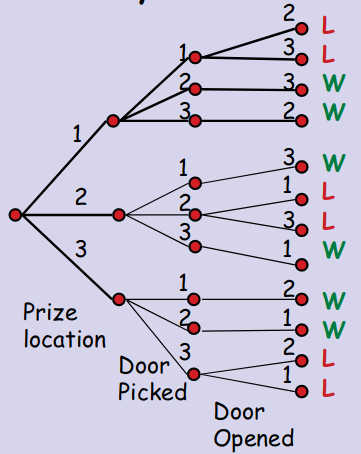
\includegraphics[width=\textwidth]{../img/monty_tree_1}

      \column{0.6\textwidth}
    
      \begin{itemize}
      \item For each step, we break down the possible outcomes.
      \item Each branch of the tree is labeled W/L
        \bigskip
        
      \item \alert{Winning outcomes:} 6
      \item \structure{Losing outcomes:} 6
        \bigskip

      \item<2> Since the \# of winning outcomes and losing outcomes
        is the same, \alert{both strategies are the same.}\\ \hfill
        (This is a {\bf Bad Conclusion})
      \end{itemize}
    \end{columns}
  }
\end{frame}

\begin{frame}
  \frametitle{Analysis: Bad Conclusion}

  {\large

    ``Since the number of winning outcomes (6) and losing outcomes (6)
    is the same, then stick strategy and switch strategy are the
    same''

    \bigskip

    \alert{Another way:} ``After door opening, one goat and one prize
    are left. The probability of being at the goat door or prize door
    is the same''

    \bigskip

    \alert{{\bf Problem}: Outcomes do not have the same probability}
  }
\end{frame}

\begin{frame}
  \frametitle{Outcomes with variable probability}

  {\large
    \begin{columns}
      \column{0.4\textwidth}
      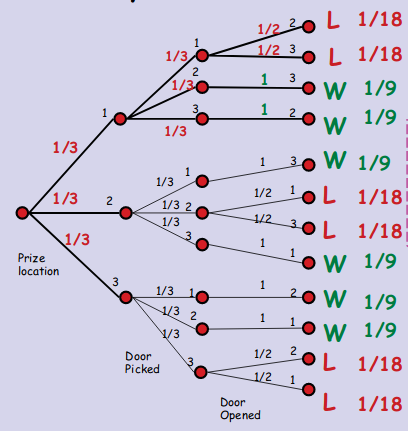
\includegraphics[width=\textwidth]{../img/monty_tree_2}

      \column{0.6\textwidth}
    
      \begin{itemize}
      \item We can assign probabilities for each of the events in
        the probability tree.
      \item By counting the probabilities of the branchs, we can
        figure out the probability of the leaves.

        \bigskip

      \item Although there are six wins, and six losses, if we compare
        the total probabilities:
      \item \structure{Total Win probability}: 6/9
      \item \alert{Total Loss probability}: 3/9
        
      \end{itemize}
    \end{columns}
  }
\end{frame}

\begin{frame}
  \frametitle{Conclusion}
  \begin{center}
    {\larger
      \alert{Switch} is better than \structure{Stick}

      \bigskip

      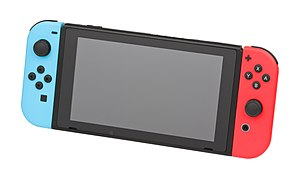
\includegraphics[width=0.35\textwidth]{../img/switch}
      \hspace{2cm}
      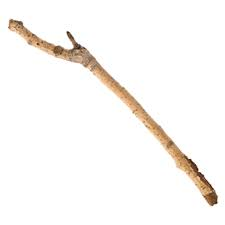
\includegraphics[width=0.35\textwidth]{../img/stick}
    }
  \end{center}
\end{frame}

\subsection{4-part Method}

\begin{frame}
  \frametitle{4-part method for calculating probabilities:}

  {\large
    \begin{enumerate}
    \item Identify the outcomes \structure{(tree helps)}
    \item Identify the event \structure{(winning)}
    \item Assign the outcome probabilities
    \item Compute the probability of the event \structure{(add it up)}
    \end{enumerate}

    \bigskip

    Avoid intuition in Probabilities!
  }  
\end{frame}

\subsection{Probability Spaces}

\begin{frame}
  \begin{center}
    {\huge
      Probability Spaces
    }
  \end{center}
\end{frame}

\begin{frame}
  \frametitle{Probability Spaces}

  {\large
    \begin{itemize}
    \item \structure{Sample Spaces}: a {\bf countable} set $S$ where the
      elements are \structure{outcomes};
      \bigskip

    \item \structure{Probability Function:} $\text{Pr}: S \to
      \{0,1\}$ so that:
      \begin{equation*}
        \sum_{\omega \in S}\text{Pr}(\omega) = 1
      \end{equation*}

      \bigskip
    \item The probability function defines the probability of each
      outcome in the Sample Space $S$.
      \bigskip

    \end{itemize}
  }
\end{frame}

\begin{frame}
  \frametitle{Probability Spaces and the Tree Model}

  {\larger The Tree Model presented in the previous example serves to
    help transforming the problem description into the probability
    space.
    \bigskip

    \begin{itemize}
    \item {\bf Outcomes}: Leaves of the tree
    \item {\bf Outcome Probabilities}: Calculated from Branch probabilities
    \end{itemize}

  }
\end{frame}

\begin{frame}
  \frametitle{Probability Spaces}

  {\large
    \begin{itemize}
    \item \structure{Sample Spaces}: a {\bf countable} set $S$ where the
      elements are \structure{outcomes};
      \bigskip

    \item \structure{Probability Function:} $\text{Pr}: S \to
      \{0,1\}$ so that:
      \begin{equation*}
        \sum_{\omega \in S}\text{Pr}(\omega) = 1
      \end{equation*}
      \bigskip

    \item \structure{Event}: A subset $E \subseteq S$
      \begin{equation*}
        \text{Pr}(E) = \sum_{\omega \in E} \text{Pr}(\omega)
      \end{equation*}
      \bigskip
      
    \item {\bf Corolary:} The sum rule
      
    \end{itemize}
  }
\end{frame}

\begin{frame}
  \frametitle{The Sum Rule}

  {\large
    For \structure{pairwise disjoint} events $A_0, A_1, \ldots$,
    \bigskip
    $\text{Pr}(A_0 \cup A_1 \cup \ldots) =
    \text{Pr}(A_0)+\text{Pr}(A_1) + \ldots$
    \bigskip

    \begin{equation*}
      \text{Pr}(\cup_{i\in\mathbb{N}}A_i) = \sum_{i\in\mathbb{N}}\text{Pr}(A_i)
    \end{equation*}

    \bigskip

    \alert{Discrete} spaces = \structure{Countable} spaces\\
    Allows the use of \structure{Sums} instead of \alert{Integrals}
    
  }
\end{frame}

\begin{frame}
  \frametitle{Generalized Probability Rules}

  {\large
    \begin{itemize}
    \item \structure{Difference Rule}: Pr$(A-B)$ = Pr$(A)$ - Pr$(A \cap B)$
      \bigskip
      
    \item<2-> \structure{Inclusion-Exclusion}: Pr$(A\cup B)$ = Pr$(A)$ + Pr$(B)$ - Pr$(A\cap B)$
      \bigskip

    \item<3-> \structure{Union Bound}: Pr$(A\cup B) \leq$ Pr$(A)$ + Pr$(B)$
      \bigskip
      
    \item<4-> \structure{Boole's Inequality}:
      $\text{Pr}(\cup_{i\in\mathbb{N}}A_i) \leq
      \sum_{i\in\mathbb{N}}\text{Pr}(A_i)$

      
    \end{itemize}

    \vfill
    
    Note how similar these rules are to the {\bf Rules of set size}
  }  
\end{frame}

\subsection{Infinite Probability}

\begin{frame}
  \frametitle{QUIZ: A Coin Game}

  {\large
    {\bf GAME:} Two players flip the same, \structure{fair} coin.

    \bigskip
    
    \begin{itemize}
    \item What is the
      probability that the \alert{first player wins}?
      \bigskip
      
    \item What is the probability that no player wins?
    \end{itemize}

  }
\end{frame}

\begin{frame}
  \frametitle{QUIZ: A Coin Game}

  {\large
    {\bf GAME:} Two players flip the same, \structure{fair} coin.

    \begin{center}
      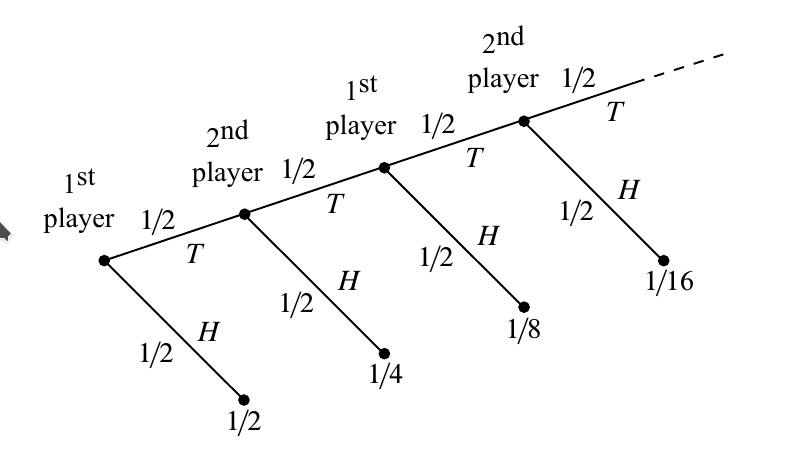
\includegraphics[width=0.6\textwidth]{../img/coin_tree}
    \end{center}

    \begin{itemize}
    \item<2-> Pr(First Player Wins) = $\frac{1}{2} + \frac{1}{8} + \frac{1}{32} + \ldots$
    \item<3-> Pr(First Player Wins) =
      $\frac{1}{2}\sum_{n=0}^{\infty}(\frac{1}{4})^n =
      \frac{1}{2}\cdot\frac{1}{1-1/4} = \frac{2}{3}$
    \end{itemize}
  }
\end{frame}

\begin{frame}
  \frametitle{Strange Dice}

  {\large

    \begin{itemize}
    \item Dice A: \{2,6,7\}
    \item Dice B: \{1,5,9\}
    \item Dice C: \{3,4,8\}
    \end{itemize}

    \begin{itemize}
    \item Game 1: You roll one dice, I roll another. Which dice wins?
    \item Game 2: You roll one dice 2 times and add. I roll one dice 2
      times and add. Which dice wins?
    \end{itemize}
  }

\end{frame}

\section{Conditional Probability}

\begin{frame}
  \frametitle{Conditional Probability: Definitions}

  {\large
    Probability that one event occurs, given that another event
    occurred.

    \bigskip

    \begin{itemize}
    \item What is the probability that a person will have a health
      problem, given their health history?
      \bigskip
      
    \item What is the probability that a stock will rise, given past
      price?
      \bigskip

    \item What is the probability that a server will overload, given
      the number of requests?
    \end{itemize}
  }
\end{frame}

\begin{frame}
  \frametitle{Conditional Probability: A fair dice example}

  {\large

    Probability of rolling a 1 in a D6.
    \begin{equation*}
    \text{Pr(Roll 1)} = \frac{|\{1\}|}{|\{1,2,3,4,5,6\}|} =
    \frac{1}{6}
    \end{equation*}

    \bigskip
    \structure{``Knowledge'' changes probabilities}\\
    Pr(Roll 1, knowing that the result was odd):
    \begin{equation*}
      \frac{|\{1\}|}{|\{1,3,5\}|} =
    \frac{1}{3}
    \end{equation*}
  }
\end{frame}

\begin{frame}
  \frametitle{Fair dice and the Tree Model}
  \begin{center}
    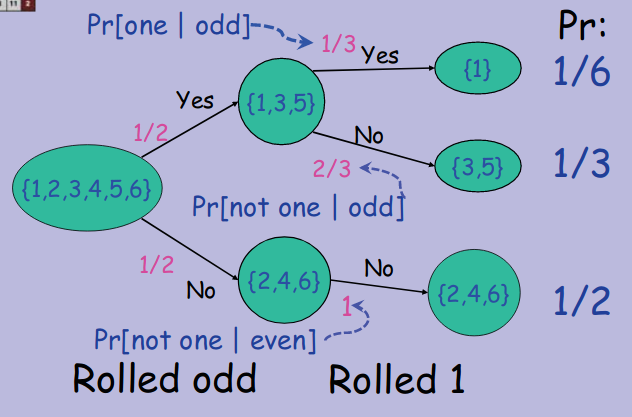
\includegraphics[width=0.8\textwidth]{../img/roll_1}
  \end{center}
\end{frame}

\begin{frame}
  \frametitle{Conditional Probability and the Tree Model}

  \begin{columns}
    \column{0.5\textwidth}
    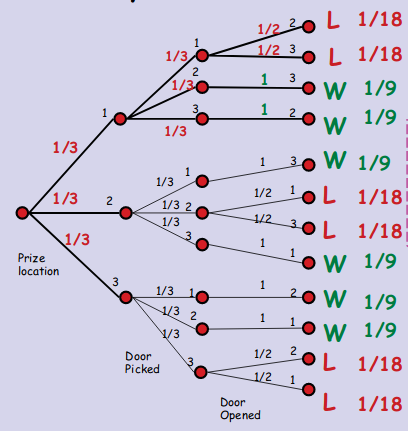
\includegraphics[width=1\textwidth]{../img/monty_tree_2}
    \column{0.5\textwidth}
      {\large
        The tree's edges are the conditional probabilities!
        \bigskip

        \begin{itemize}
        \item Pr(pick 1|prize 1) = 1/3
        \item Pr(pick 2|prize 3) = 1/3
          \bigskip
          
        \item Pr(open 3|prize 1 \& pick 1) = 1/2\\
          We can compose conditional probs!
          
        \end{itemize}
      }
  \end{columns}
  \only<2>{The tree model was using conditional probabilities implicitely!}
\end{frame}

\begin{frame}
  \frametitle{Probability: Product Rules}

  {\large
    What is the probability that \alert{both} A \& B happen?

    \begin{equation}
      \text{Pr}(A\cap B) = \text{Pr}(A) \cdot \text{Pr}(B|A)
    \end{equation}
    \bigskip
    
    This implies a \structure{definition of conditional Prob:}
    \begin{equation}
      \text{Pr}(B|A) ::= \frac{\text{Pr}(A\cap B)}{\text{Pr}(A)}
    \end{equation}

  }
\end{frame}

\begin{frame}
  \frametitle{Conditional Probability as a Probability Space}

  {\large
    \structure{Another way to think} about conditional probability is
    that, when we define a probability conditional to A, we
    \alert{create a new probability space} where all events not following
    A have a probability of 0.

    \vfill

    Let Pr$_A$ be the probability function conditional to $A$, then:
    \begin{equation*}
      \text{Pr}_A(\omega) = 0, \text{ if } \omega \notin A
    \end{equation*}
    \begin{equation*}
      \text{Pr}_A(\omega) = \frac{\text{Pr}(\omega)}{\text{Pr}(A)},
      \text{ otherwise.}
    \end{equation*}

  }
\end{frame}

\begin{frame}
  \frametitle{Conditional Probability: Quiz}

  {\large
    Imagine that I roll \structure{two} dice, and the sum is a \structure{four}.
    What is the probability that \alert{one of the dice is a 3}?

    \vfill
    
    \begin{itemize}
    \item<2-> Total Events: (1,1),(1,2),(1,3),$\ldots$,(6,5),(6,6)
    \item<3-> Events when sum = 4: (1,3), (2,2), (3,1)
    \item<4-> Events when dice = 3 \& sum = 4: (1,3), (3,1)
      \bigskip

    \item<5-> Probability: 2/3
    \end{itemize}
    
  }
\end{frame}

\subsection{Bayes' Theorem}
\begin{frame}
  \frametitle{A 99\% accurate TB testing}

  {\alert

    {\bf Imagine} a great looking test for Tuberculosis:
    \begin{itemize}
    \item If you \alert{have TB}, the test is always \structure{correct}
    \item If you \alert{don't have TB}, the test is correct \structure{99\% of the time}
      \bigskip

    \item<2-> The doctor does this test \alert{and says you have TB!}
    \item<2-> The test is 99\% accurate!
    \item<2-> Recently, many antibiotics don't worry anymore!
      \bigskip

    \item<3> Should you worry?      
    \end{itemize}
  }
\end{frame}

\begin{frame}
  \frametitle{99\% diagnostic test and conditional probability}

  {\large

    What is the \structure{probability that you have TB}, if the \%99
    accuracy test says \alert{Yes}?
    \begin{equation*}
      \text{Pr(TB | test positive)} = ?
    \end{equation*}

    \bigskip

    What do we know about this test?
    \begin{itemize}
    \item<2-> Pr(Positive | \structure{TB}) = 1
    \item<2-> Pr(Positive | \alert{Not TB}) = 1/100
      \bigskip

    \item<3-> \alert{False Positive Rate} = 1\%
    \end{itemize}
  }
\end{frame}

\begin{frame}
  \frametitle{Do you have TB or Not?}

  {\large
    \begin{itemize}
    \item Definition of \structure{Conditional Probability}:
    \item Pr(TB | Positive) = $\frac{\text{Pr(Positive and TB)}}{\text{Pr(Positive)}}$
      \bigskip

    \item<2-> Pr(TB | Positive) = $\frac{\text{Pr(Positive | TB)}\cdot\text{Pr(TB)}}{\text{Pr(Positive)}}$
    \item<2-> Pr(TB | Positive) = $\frac{1\cdot\text{Pr(TB)}}{\text{Pr(Positive)}}$ = $\frac{\text{Pr(TB)}}{\text{Pr(Positive)}}$
      \bigskip

    \item<3-> Pr(Positive) = ?
    \item<3-> By the \structure{Total Probability formula}:
    \item<3-> Pr(Positive) = Pr(Positive | TB)$\cdot$Pr(TB) + Pr(Positive | Not TB)$\cdot$Pr(Not TB)
    \item<4-> Pr(Positive) = $1\cdot$Pr(TB) + $\frac{1}{100}\cdot$Pr(Not TB)
    \end{itemize}    
    
  }
\end{frame}

\begin{frame}
  \frametitle{Do you have TB or Not?}

  {\large
    \begin{itemize}
    \item \structure{Conditional Probability}:
    \item Pr(TB | Positive) = $\frac{\text{Pr(TB)}}{\text{Pr(Positive)}}$
      \bigskip

    \item<2-> Pr(Positive) = $1\cdot$Pr(TB) + $\frac{1}{100}\cdot$(1 - Pr(TB)) = 99/100 Pr(TB) + 1/100
    \item<3-> Pr(TB | Positive) = $\frac{\text{Pr(TB)}}{\text{Pr(Positive)}}$ = $100\cdot\frac{\text{100 Pr(TB)}}{99 Pr(TB) + 1}$
      \bigskip

    \item<3-> Now we need to know ``Pr(TB)''. In the United States, it
      is about 11.000 per 100 million people, or 0.001.
      \bigskip
      
    \item<4-> Pr(TB | positive) = $\frac{100/10000}{99/10000 + 1} = 1/100$
    \end{itemize}


  }
\end{frame}

\begin{frame}
  \frametitle{Conditional Probability and Tricky Base Rates}

  {\large
    \begin{itemize}
    \item Even if you have the \structure{positive diagnostic}, your chance of having TB is 1\%.
      \bigskip

    \item This is because the {\bf TB Rate (0.01\%)} is much lower
      than the {\bf False Positive Rate (1\%)}
      \bigskip

    \item So the 99\% accurate test was not so accurate here...
      \vfill

    \item This is a good example of {\bf \structure{Bayes' Rule}}
      \begin{equation*}
        \text{Pr}(B|A) = \frac{\text{Pr}(A|B)\cdot\text{Pr}(B)}{\text{Pr}(A)}
      \end{equation*}
      
    \end{itemize}

  }
\end{frame}

%%%%%%%%%%%%%%%
%% TODO: Sympsom Paradox and Independence
%%%%%%%%%%%%%%

\section{Conclusion}

\begin{frame}
  \frametitle{Probability in Computer Sciences: The Birthday Paradox}

  {\large
    \begin{itemize}
    \item In a class with 95 people, what is the probability that {\bf two
      people have a birthday in the same day}?
      \bigskip

    \item <2-> $n = 95, d = 365$.
    \item <2-> Event space is sequences of $n$ numbers with no repetitions.
      \bigskip

    \item <3-> \alert{The Birthday Principle}: When $n = \sqrt{2d}$,
      the probability of two people having the same birthday is about
      $0.632$
    \item <3-> This same principle is applied to \structure{hashing collisions}.
    \end{itemize}
  }
\end{frame}

\begin{frame}
  \frame{Class Summary}

  {\large
    \begin{itemize}
    \item We can see probability problems as counting or combinatory problems.\\
      \alert{Probability = Events of Interest / Total Events}
      
      \bigskip

    \item We can use the \structure{Tree Model} to make problems easier to understand.
      \bigskip

    \item Conditional Probability, and Bayes' Rule
    \end{itemize}
  }
\end{frame}


%%%%%%%%%%%%%%%%%
% Independence and Causality
% Random Variables and Density Functions
% Expectation

%%%%%%%%%%%%%%%%%
% Deviation: Markov and Chebyschev Bounds
% Sampling and Confidence
% Random Walks and Pagerank


\begin{frame}
  \frametitle{Image Credits}
  \begin{itemize}
  \item Poker hand photo by ``Poker Photos''
  \item Let's Make a deal photo by ``www.letsmakeadeal.com''
  \item Switch and Stick photo by Wikipedia
  \end{itemize}
\end{frame}

\end{document}
